\chapter{Realised work}


This chapter describes ...

general procedure 

<diagram flowchart>


\section{First module : image processing operations}


\subsection{Procedure}

=> est une introduction 

<diagram flowchart>


\subsection{Images}

An image is represented by a width, an heigth, colors (stocked in pixel values, i.e. positive integers), and a color model. A color model describes how the colors are represented, that is how many values should be used in order to represent a color \cite{bib:image:ColorModel}. Multiples color models exist, for example : 
\begin{itemize}
	\item RGB, where a color is represented by the three primary colors (red, green and blue)
	\item CMY, where a color is represented by a combinaison of cyan, magenta and yellow colors
\end{itemize}

% cours de jpeg 

~~

This project is dealing with three types of images : RGB, Grey and Monochromatic images. A grey image is an image where the pixels are represented in a grey scale by only one value, the grey value (which can have any integer values between 0 and 255 included). In other words, there is 256 possible colors in a grey images, which are all shade of grey. In a monochromatic image, only two colors are represented, black (with the value 0) and white (with the value 255).

~~

Once an image is loaded in the RGB color model, we converted it into a grey image in order to reduce the number of information present in the image and lower the complexity. The monochromatic image were used in order to determinate edges and extract the objects in the image.

~~

The grey value of a RGB pixel is determined by doing the average of the red, green and blue values. As for the monochromatic image, we first have to define a 
threshold value, then a pixel will be represented in black if it's grey value is strictly under the threshold, and in white otherwise (the equation \ref{eq:threshold} show it in a more mathematical point of view) \cite{bib:image:Threshold}.

\begin{equation} \label{eq:threshold}
mono_{threshold}(greyValue) = 
	\begin{cases}
		BLACK & \text{if } greyValue < threshold \\
		WHITE & \text{otherwise} \\ 
	\end{cases}
\end{equation}


%We choosed to represent the grey and monochromatic image by a one matrix. 
%.... 
%<changer RGB image> 
%~~

\begin{figure}
	\centering 
	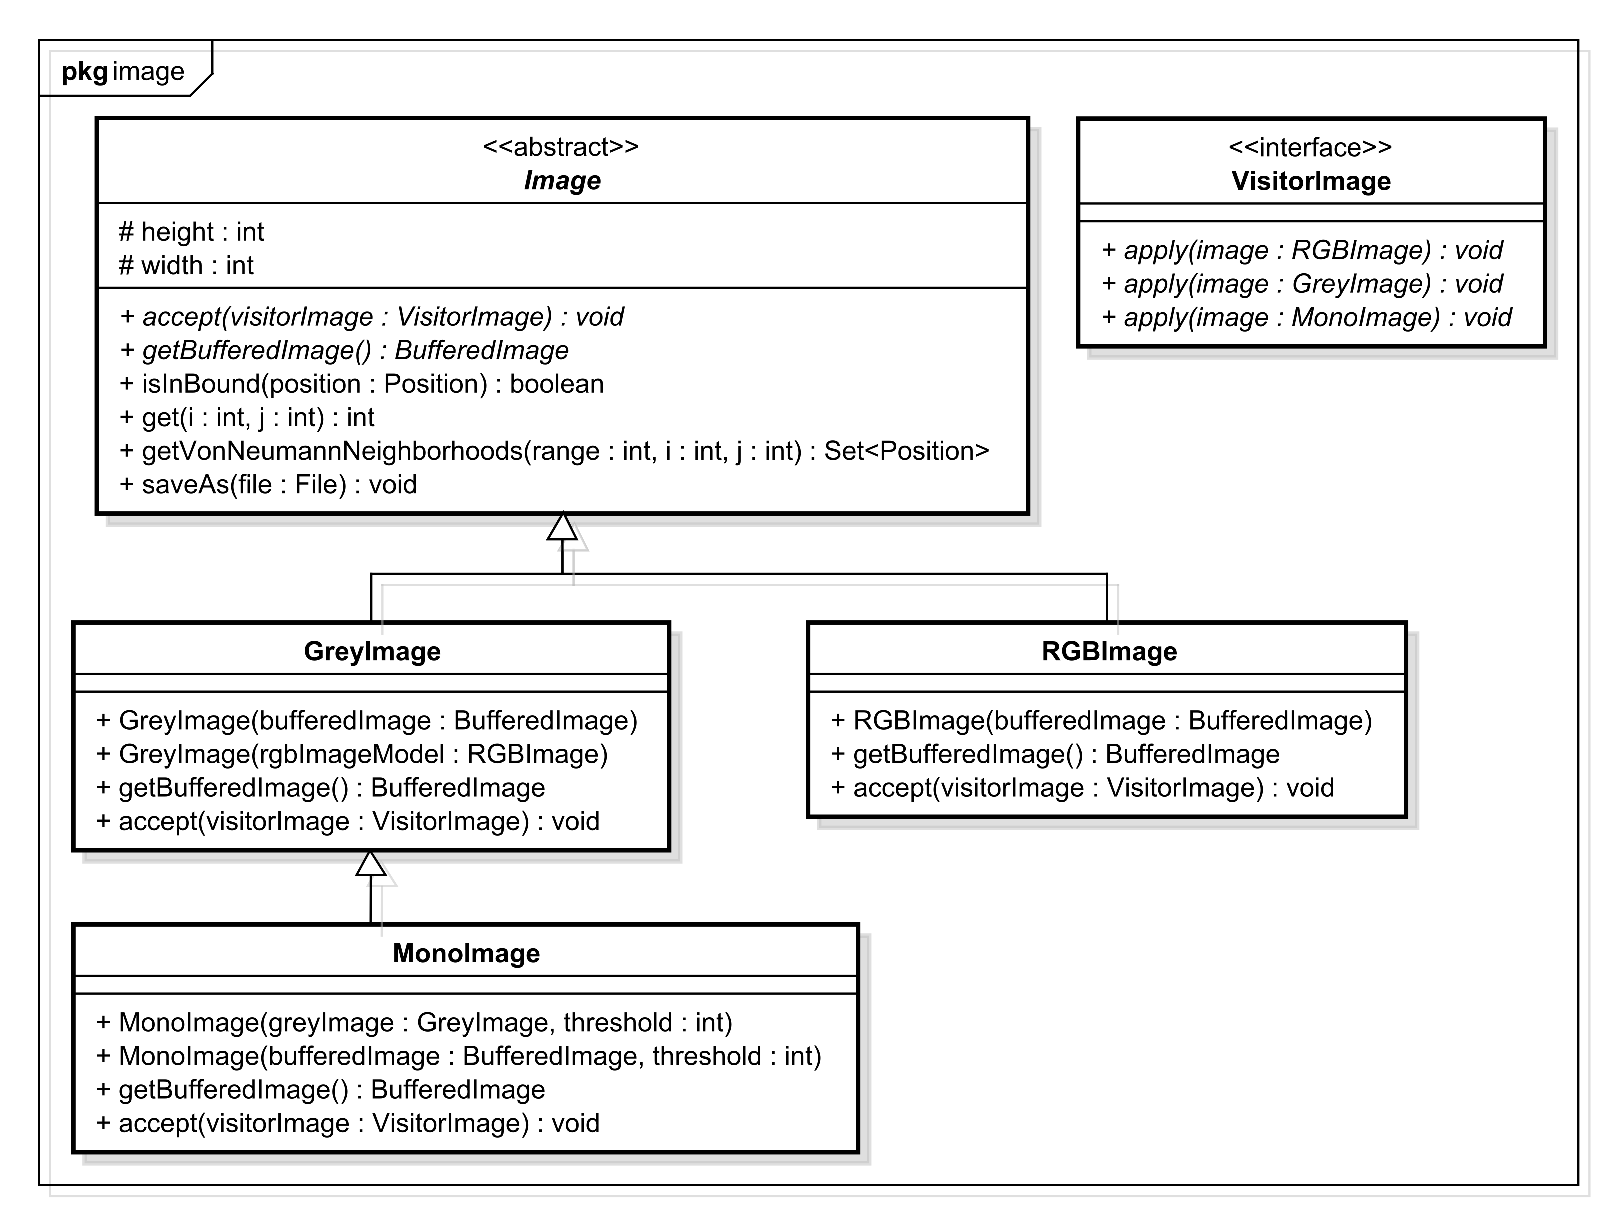
\includegraphics[width=0.75\textwidth]{images/diagrams/class_diagram_image}
	\caption{Image package class diagram}
	\label{fig:diagram:class:image}
\end{figure}

The \vref{fig:diagram:class:image} shows the class diagram that was used. The visitor pattern was also used in order to facilitate the implementation of new processes (or algorithms) on a data structure without changing it. It does so by separating the algorithm and the data structure from each other. A new process (or algorithm) could be added by extending the VisitorImage class and implementing the apply method for each image subclasses \cite{bib:pattern:Visitor}. 

% + cours 
% + book

~~

The axis we used to represent an image are illustrated on the \vref{fig:axis representation}. 

\begin{figure}[h]
	\centering
	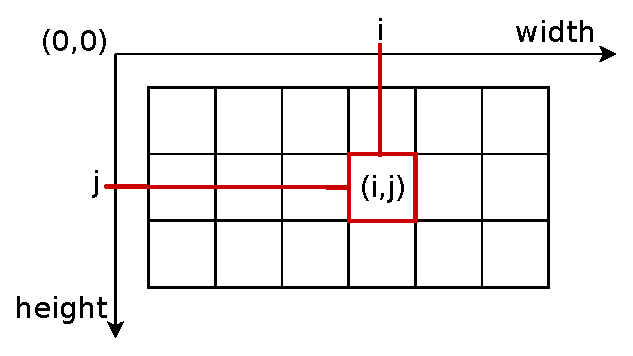
\includegraphics[width=0.5\textwidth]{images/axis/axis_representation}
	\caption{Axis representation}
	\label{fig:axis representation}
\end{figure}






\subsection{Filters}

\subsection{Cellular Automata algorithm}

\subsection{Morphology}



\subsection{GUI}

A Graphic User Interface has been developped during the project in order to see the results.... 







\section{Second module : object recognition on 2D images}




\subsection{Feature Extraction and Freeman Chain Code}


A feature is defined as something in the image that have a certain shape and edges. 

%As we said before, in order to detect the different edges in th eimage, we used a filter edge detection, like sobel or canny. 

%In order to extracts the differents features in the image, 




\subsubsection{Freeman Chain Code and it's extraction}

The Freeman Chain Code is a coding edge algorithm. It allows to represent a shape given in a bimary image (monochromatic) by it's edge. It's first purpose is to compress the data, as we pass from a binary image to a chain (or list) of code representing the shape of the edge \cite{bib:chain:ParametreGeometriqueChaineFreeman}. In other words, it's a data structure for representing the boundary of a feature \cite{bib:chain:DigitalImageProcessing}.

~~

In order to extract the chain code of a shape in a binary image, it is necessary to start from on of the end edges. For this project, it has been decided to start from the most left upper edge point of the shape, i.e. there isn't any other edge point that is at the left of the starting point. In order to have this starting point, the image has been travelled from up to down, and then from left to right, as it is shown on the \vref{fig:chain code:course order}.

\begin{figure}[H]
	\centering
	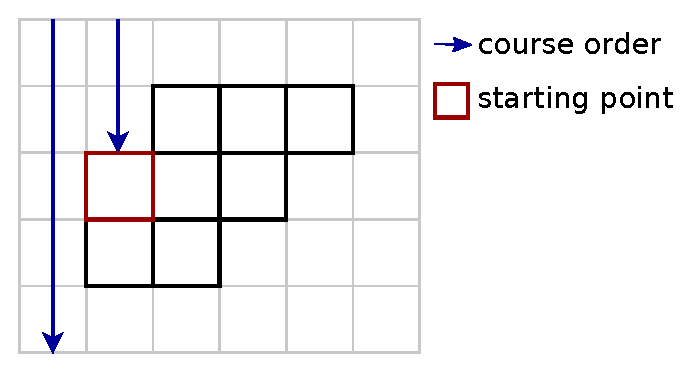
\includegraphics[width=0.5\textwidth]{images/chain_code/course_order}
	\caption{Course order of the binary image \cite{bib:chain:ParametreGeometriqueChaineFreeman}}
	\label{fig:chain code:course order}	
\end{figure}

Once the starting point is determined, it is then possible to follow the boundary in the anticlockwise direction. Then, depending on the direction, a code is generated according to the following direction scheme illustrated with the \vref{fig:chain code:direction scheme star}, where the central point of the star represent the current boundary pixel. For example, if the next boundary pixel is on the top of the current one, the code 2 will be generated. 


\begin{figure}[H]
	\centering
	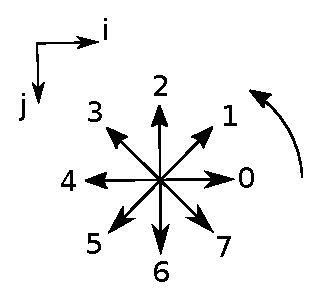
\includegraphics[width=0.2\textwidth]{images/chain_code/direction_scheme_star}
	\caption{Direction scheme star \cite{bib:chain:ParametreGeometriqueChaineFreeman}}
	\label{fig:chain code:direction scheme star}	
\end{figure}


Moreover, in order to support more complexe shapes, the pixel neibors of the current boundary pixel are travelled depending on the last generated code (i.e. on the last direction). In other words, the stating point of the star is changed depending on the last direction. The first pixel neibor that should be visited must be the previous pixel boundary (i.e. the origin of the direction used to get on the current pixel). 

~~

For example, the chain code "6011445" can be produced with the shape given on the \vref{fig:chain code:course order}. The \vref{fig:chain code:example} explains the procedure. 
\begin{figure}[H]
	\centering
	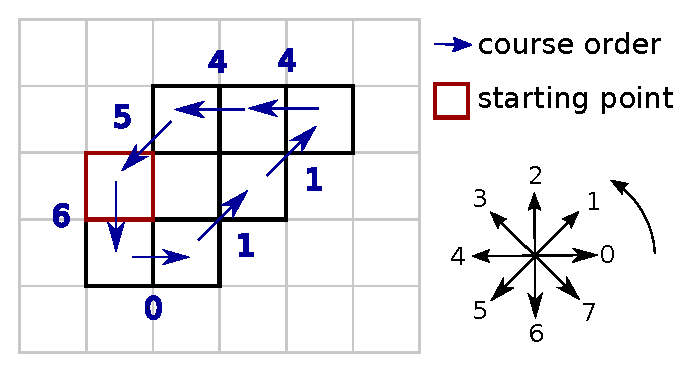
\includegraphics[width=0.5\textwidth]{images/chain_code/example}
	\caption{Example of a chain code}
	\label{fig:chain code:example}	
\end{figure}

~~

Chain codes are translation invariant but depend on rotation, which mean that differents chain codes will be produced for the shape and it's rotation. It is possible to make the chain code invariant to rotation by using the fisrt difference of the chain code instead, i.e. each code will be substracted with the previous code modulo 8 (as we are in 8-connexity). The new chain will be named differential chain code \cite{bib:chain:RepresentationAndDescription}. The calculation of the differential chain code of the shape of the \vref{fig:chain code:course order} is given with the \vref{tab:chain code:differential chain code}.
\begin{equation} \label{eq:chain code:differential chain code}
d_i = code_i - code_{(i-1) \bmod N} \bmod 8
\end{equation}

%%%%%%%%%%%%%%%%%%%%%%%%%%%%%%%%%%%%%%%
\begin{comment}
	\begin{cases}
		code_i - code_{i-1} mod 8 & \text{if } i \not = 1 \\
		code_i - code_{N} mod 8 & \text{otherwise} \\
	\end{cases}
\end{comment}
%%%%%%%%%%%%%%%%%%%%%%%%%%%%%%%%%%%%%%%


\begin{table}[h]
	\centering
	\caption{Example of a differential chain code}
	\label{tab:chain code:differential chain code}
	\begin{tabular}{rccccccc}
\toprule 
chain code   & 6     & 0     & 1     & 1     & 4     & 4     & 5     \\
substraction & 6 - 5 & 0 - 6 & 1 - 0 & 1 - 1 & 4 - 1 & 4 - 4 & 5 - 4 \\
value     	 & 1     & -6    & 1     & 0     & 3     & 0     & 1     \\
modulo 8 (differential code)  	 & 1     & 2     & 1     & 0     & 3     & 0     & 1     \\ 
\bottomrule 
	\end{tabular}
\end{table}


% http://poseidon.csd.auth.gr/LAB_PUBLICATIONS/Books/dip_material/chapter_7/chap7en.pdf 
% http://www.ece.uvic.ca/~aalbu/computer%20vision%202009/Lecture%2022.%20Shape%20description-contours.pdf 
% http://www.vis.uky.edu/~ryang/teaching/cs635-2016spring/Lectures/16-representation.pdf 

\subsubsection{Feature Extraction}


After extracting the chain code from a shape, it is then possible to extracts features from it. A feature is another piece of information or characteristic which is relevent for solving a task \cite{bib:extraction:definition}. The following features were extracted : 
\begin{itemize}
	\item the perimeter (the number of boundary pixels)
	\item the area, which is the number of pixels in the region or shape 
	\item the width and the height 
	\item the compactness 
	\item the circularity 
	\item the curvature, representing the successive changes in directions 
	\item the bending energy 
\end{itemize}

~~ 

The perimeter can be calculated using the following \vref{eq:feature extraction:perimeter}. $n_e$ represents the number of even chain elements (i.e. code), and $n_o$ the number of odd chain elements \cite{bib:chain:EstimateAreasAndPerimetersChainCode}. Others equations improve the perimeter length estimation, like the \vref{eq:feature extraction:kulpa} given by Kulpa which is used in this project \cite{bib:chain:ObjectDescription}.
\begin{align} 
P &= n_e + \sqrt{2}*n_o \label{eq:feature extraction:perimeter} \\
P_K &= \frac{\pi}{8} * (1 + \sqrt{2}) * P \label{eq:feature extraction:kulpa}
\end{align}
% http://www.mva-org.jp/Proceedings/CommemorativeDVD/1994/papers/1994272.pdf 
% https://www.uio.no/studier/emner/matnat/ifi/INF4300/h15/undervisningsmateriale/inf4300-2015-f06-description.pdf 


~~

The width and height can be calculated by knowing the chain code values, and thanks to the direction shape star (\vref{fig:chain code:direction scheme star}). As the chain code should return to the starting point, there is the same number of displacements from the left to the right and from the right to the left. It is then possible to calculate the width by counting the number of displacement from one direction (e.g. from the left to the right), which can be known by using thedirection shape star values. The same goes for the height. The following equations illustrate the process, where $N$ is the number of elements (or code) in the chain code, and $code_i$ is the i$^{th}$ element of the chain code \cite{bib:chain:ShapeDescription}.
\begin{align}
width &= \sum_{i = 1}^{N} w_i 
& \text{ with } w_i = 
	\begin{cases}
		1 & \text{if } code_i = 0, 1, 7 \\
		0 & \text{otherwise} \\
	\end{cases} \\
height &= \sum_{i = 1}^{N} h_i 
& \text{ with }  h_i = 
	\begin{cases}
		1 & \text{if } code_i = 5, 6, 7 \\
		0 & \text{otherwise} \\
	\end{cases} 
\end{align}

% \label{eq:feature extraction:compactness} 

~~

The compactness is calculated with the following \vref{eq:feature extraction:compactness}. It is invariant to translation, rotation and scale  \cite{bib:chain:RepresentationAndDescription}.
\begin{equation} \label{eq:feature extraction:compactness}
compactness = \frac{perimeter^2}{area}
\end{equation}

~~

The circularity ratio is given by the \vref{eq:feature extraction:circularity}. It is equal to 1 when the shape is a perfect continuous circle and between 0 and 1 for other shapes \cite{bib:chain:ObjectDescription}.
\begin{equation} \label{eq:feature extraction:circularity}
circularity = \frac{4 * \pi * area}{perimeter^2}
\end{equation}

~~ 

The curvature is the change of rate of slope \cite{bib:chain:ObjectDescription}, in other words it is the ratio between the number of direction changes and the total number of boundary pixels. It can be obtained by summing the elements of the shape differencial chain code  \cite{bib:chain:ShapeRepresentationDescription}. In the following equation, $N$ represents the number of the chain code elements, and $diffCode_i$ represents the i$^{th}$ element of the differential chain code. 
\begin{equation}
curvature = \sum_{i = 0}^{N} \text{diffCode}_i
\end{equation}

% http://www.cb.uu.se/~ingela/Teaching/ImageAnalysis/Shape2002.pdf 
% bib:chain:ShapeRepresentationDescription 

~~

The bending energy is calculated by integrating the squared curvature along the entire contour of the shape \cite{bib:chain:ShapeRepresentationDescription}. According to \cite{bib:chain:ShapeDescriptionLesson}, it is a good feature for shape matching. 
\begin{equation}
bendingEnergy = \frac{1}{N} \sum_{i = 0}^{N} (\text{diffCode}_i)^{2}
\end{equation}


\subsubsection{Modelisation}










\subsection{The database creation}

The database purposes is to store the known tagged objects. It has been decided that those objects will be stores through their features. The database was created with Oracle Database, which contains only one table named "AnnotatedObjects". This table stores the information regarding the tagged objects, which is an id and the tagged object's features (as shown in the previous section).

~~

The \gls{DAO} pattern is used in order to facilitate the access to the database. The \gls{DAO} pattern allows to differentiate the data to be accessed, and the way they are stored. To do so, it separate the business object (in a bean package), how the data are recovered (in a dao package, i.e. the requests), and the storage system (in a session package). For each table in the database, there must be one bean class to store the values and one dao class to access it, nammed after the table's name. Moreover, as it is not necessary to have more than one instance of each dao classes per sessions, a factory pattern is used to store singleton instances of each created dao per session, and to return it when needed.

%diagramme de classe à expliquer 
~~


The \vref{fig:diagram:class:database} displays the class diagram of the database package. An abstract Session class provides a general way of connecting to a database, regarding of the user's id, the database's url, and the \gls{DBMS} used (e.g. Oracle, MySQL). A general abstract DAO class also provide basis requests to be implemented. When a new table is added into the database, it is necessary to create a new bean class, a new dao class by extending the abstract class "DAO", and add a method in the factory in order to be able to access the new dao class.


\begin{figure}[h]
	\centering 
	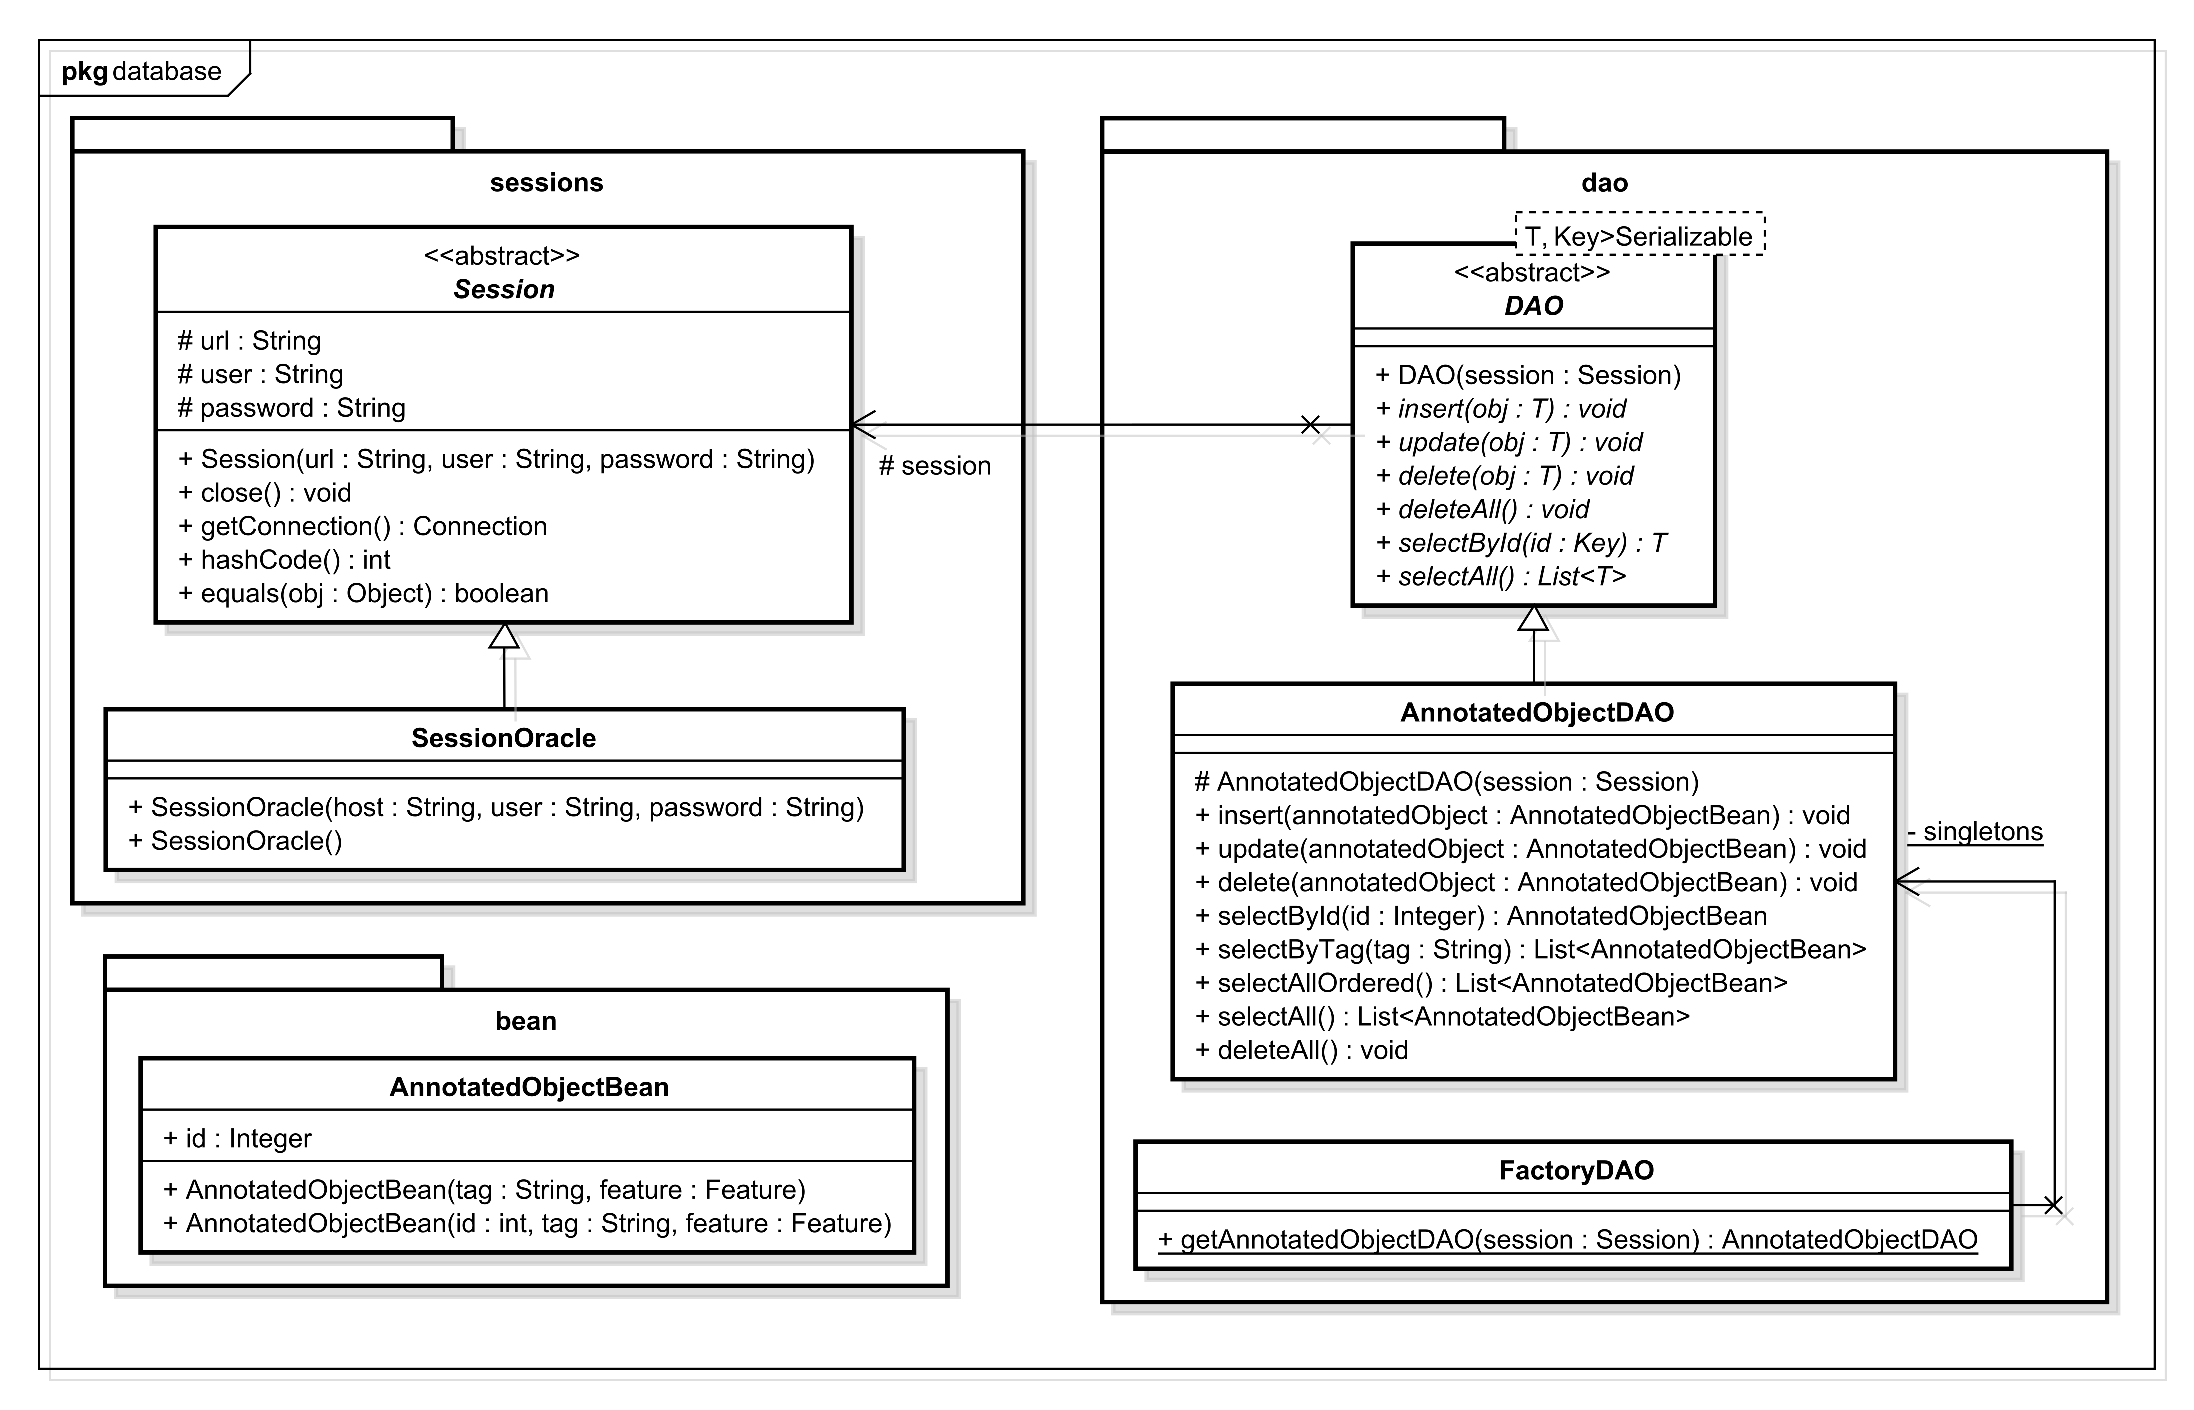
\includegraphics[width=1\textwidth]{images/diagrams/class_diagram_database}
	\caption{Database package class diagram}
	\label{fig:diagram:class:database}
\end{figure}


\subsection{The selected dataset}

Multiple dataset can be found on the Internet, for example the \href{http://groups.csail.mit.edu/vision/SUN/}{SUN database}, the \href{http://cbcl.mit.edu/software-datasets/streetscenes/}{StreetScenes framework}, the \href{http://host.robots.ox.ac.uk/pascal/VOC/voc2007/index.html}{PASCAL Visual Object Classes} and the \href{http://labelme2.csail.mit.edu/Release3.0/browserTools/php/dataset.php}{LabelMe dataset}. For this project, it has been chosen to use the last one, the LabelMe dataset, has it seems to be the most suited to the project needs. LabelMe was created by the MIT Computer Science and Artificial Intelligence Laboratory, it's goal is to provide an online annotation tool in order to build image databases for computer vision research. An application was released on the 10$^{th}$ of December 2012 for iPhone and iPad \cite{bib:labelme}.

~~

LabelMe represents the extracted objects in the form of polygons, stored in a xml file. Each annotated images in associated to one xml file, which contains every annotated objects present in that image. For retrieving the dataset (i.e. the images and their annotations), LabelMe provide a Matlab toolbox, which allow to customize to portion of the database the user want to access (i.e. by giving the folders, tags, etc.). As describes in the LabelMe documentation, it is possible to access the dataset either by downloading all the interested images locally and then explore the dataset, or access the dataset online and exlore it before downloading what is necessary. The first method is advised by LabelMe authors, but seems to bug during the downloading of the dataset. The second method was used, Matlab scrips were written in order to specify the folders to explore, which tagged object to recover (by giving the tag), and the local folder were the annotations should be saved.

~~

In order to save the annotated objects from the xml files to the database, a xml parser is used to travel the xml files and get each annotated object through his tag and the polygon. Then the features of the polygon are extracted with the same methods as the chain code, and are stored into the database by using the dao. As for parsing the xml files, the \acrshort{SAX} is used. 

% création d'un parseur xml pour extraire les données


\subsection{Tagging}

% comparer chaque champs un par un 
% donner l'ordre des champs 

% ordre de préférence (d'abord lui, puis lui, puis lui...)
% utilisation de comparator pour pouvoir comparer les obj via leurs features
% - un comparator par featur 
% - un comparator global utilisant les autres comparator dans un ordre spécific

% récupération des obj annoté de la db via dao
% trouver l'obj annoté le plus proche de l'objet à annoter
% - ordoner les obj annoté du plus petit au plus grand via l'instruction 'order by' de la requete sql
% - utilisation du quicksort pour obtenir un interval dans lequel l'obj le plus proche se trouve
% - comparer les trois derniers objets (les obj annoté de l'interval), lequel est vraiment le plus proche de l'obj à annoter




\subsection{Classification with K-means algorithm}

Some definitions related to \gls{data analysis} and \gls{classification} area can be found in the glossary section. The K-means \gls{algorithm} is a non-hierarchical \gls{classification} \gls{algorithm} (i.e. during the \gls{classification}, no hierarchy between \glspl{individual} is used). For this project, it has been decided to implement the K-means \gls{algorithm} instead of the \gls{EM} because K-means shows better results. 

~~ 

The principle of K-means is the following (\cite{bib:clustering:AnalyseDesDonnees}). First, $n$ \glspl{individual} are chosen to be the initial gravity center of each \glspl{cluster} (where $n$ is the number of clusters). Then, each individual is affected (added) to the nearest \gls{cluster} by comparing the \gls{individual} and the \gls{cluster}'s gravity center, the \gls{cluster}'s gravity center is then  updated accordingly. The second step is repeated until the \gls{algorithm} converge (i.e. the iteration when no \gls{individual} changes \gls{cluster}). The gravity center of each \gls{cluster} is updated each time an \gls{individual} is added or removed of the \gls{cluster}.

~~

The \vref{fig:diagram:class:kmeans} shows the class diagram used to implement the K-means \gls{algorithm}. The class Individual contains a certain number of variables. The class Cluster gathers a list of individuals with the same number of variables. After performing the classification, the K-means \gls{algorithm} will return a list of $n$ Clusters. Moreover, an array "classes" in the KMeans class stores the \gls{cluster}'s number (between $[0;n[$) affected to each \gls{individual}.


\begin{figure}[h]
	\centering 
	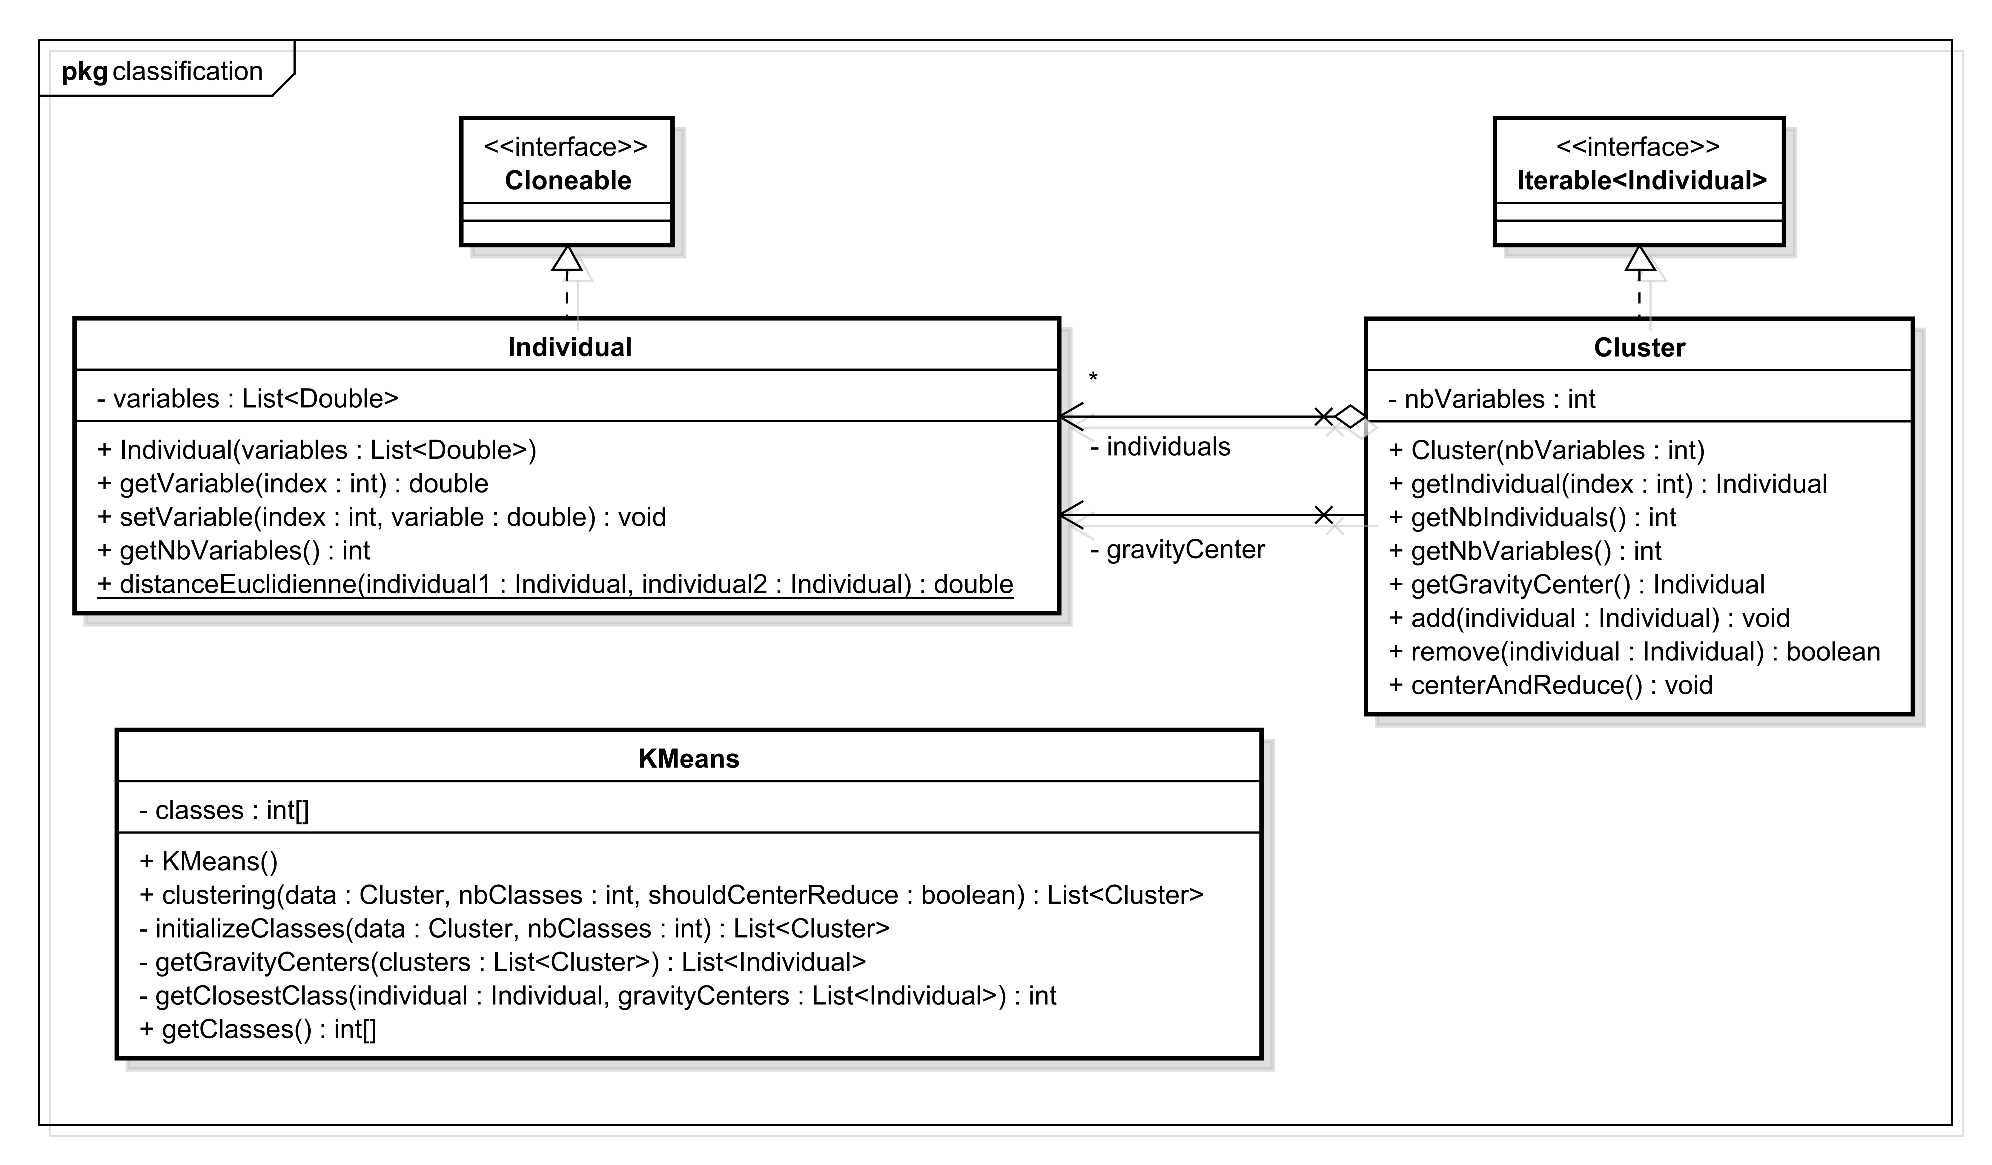
\includegraphics[width=1\textwidth]{images/diagrams/class_diagram_kmeans}
	\caption{K-means class diagram}
	\label{fig:diagram:class:kmeans}
\end{figure}



The K-means \gls{algorithm} has some defaults : 
\begin{itemize}
	\item it is necessary to know the number of clusters before the execution of the \gls{algorithm}
	\item K-means can return different results for the same input (as it chooses random \glspl{individual} for initializing the \glspl{cluster})
\end{itemize}





